%%%%%%%%%%%%%%%%%%%%%%%%%%%%%%%%%%%%%
%                                   %
% Compile with XeLaTeX and biber    %
%                                   %
% Questions or comments:            %
%                                   %
% joshua dot mcneill at uga dot edu %
%                                   %
%%%%%%%%%%%%%%%%%%%%%%%%%%%%%%%%%%%%%

\documentclass{beamer}
  % Read in standard preamble (cosmetic stuff)
  %%%%%%%%%%%%%%%%%%%%%%%%%%%%%%%%%%%%%%%%%%%%%%%%%%%%%%%%%%%%%%%%
% This is a standard preamble used in for all slide documents. %
% It basically contains cosmetic settings.                     %
%                                                              %
% Joshua McNeill                                               %
% joshua dot mcneill at uga dot edu                            %
%%%%%%%%%%%%%%%%%%%%%%%%%%%%%%%%%%%%%%%%%%%%%%%%%%%%%%%%%%%%%%%%

% Beamer settings
% \usetheme{Berkeley}
\usetheme{CambridgeUS}
% \usecolortheme{dove}
% \usecolortheme{rose}
\usecolortheme{seagull}
\usefonttheme{professionalfonts}
\usefonttheme{serif}
\setbeamertemplate{bibliography item}{}

% Packages and settings
\usepackage{fontspec}
  \setmainfont{Charis SIL}
\usepackage{hyperref}
  \hypersetup{colorlinks=true,
              allcolors=blue}
\usepackage{graphicx}
  \graphicspath{{../../figures/}}
\usepackage[normalem]{ulem}
\usepackage{enumerate}

% Document information
\author{M. McNeill}
\title[FREN2001]{Français 2001}
\institute{\url{joshua.mcneill@uga.edu}}
\date{}

%% Custom commands
% Lexical items
\newcommand{\lexi}[1]{\textit{#1}}
% Gloss
\newcommand{\gloss}[1]{`#1'}
\newcommand{\tinygloss}[1]{{\tiny`#1'}}
% Orthographic representations
\newcommand{\orth}[1]{$\langle$#1$\rangle$}
% Utterances (pragmatics)
\newcommand{\uttr}[1]{`#1'}
% Sentences (pragmatics)
\newcommand{\sent}[1]{\textit{#1}}
% Base dir for definitions
\newcommand{\defs}{../definitions}


  % Document information
  \subtitle[Social Factors]{Social Factors in Language Variation}

  %% Custom commands
  % Subsection/frame title
  \newcommand{\suboneone}{What are social factors?}
  \newcommand{\subonetwo}{Socioeconomic class}
  \newcommand{\subonethree}{Age}
  \newcommand{\subonefour}{Gender}
  \newcommand{\subonefive}{Ethnicity}

\begin{document}
  % Read in the standard intro slides (title page and table of contents)
  %%%%%%%%%%%%%%%%%%%%%%%%%%%%%%%%%%%%%%%%%%%%%%%%%%%%%%%%%%%%%%%%
% This is a standard set of intro slides used in for all slide %
% documents. It basically contains the title page and table of %
% contents.                                                    %
%                                                              %
% Joshua McNeill                                               %
% joshua dot mcneill at uga dot edu                            %
%%%%%%%%%%%%%%%%%%%%%%%%%%%%%%%%%%%%%%%%%%%%%%%%%%%%%%%%%%%%%%%%

\begin{frame}
  \titlepage
  \tiny{Office: % Basically a variable for office hours location
Gilbert 121\\
        Office hours: % Basically a variable for office hours
 lundi, mercredi, vendredi 10:10--11:10
}
\end{frame}

\begin{frame}
  \tableofcontents[hideallsubsections]
\end{frame}

\AtBeginSection[]{
  \begin{frame}
    \tableofcontents[currentsection,
                     hideallsubsections]
  \end{frame}
}


  \section{Social Factors}
    \subsection{\suboneone}
      \begin{frame}{\suboneone}
        \begin{block}{These people likely wouldn't speak the same}
          \begin{enumerate}
            \item A \alert<2>{20 year old}, \alert<4>{white}, \alert<1>{working-class} \alert<3>{female} from Georgia in a casual conversation
            \item A \only<2>{\alert{60 year old}}\only<1,3->{20 year old}, \only<4>{\alert{African-American}}\only<1-3>{white}, \only<1>{\alert{upper-class}}\only<2->{working-class} \only<3>{\alert{male}}\only<1-2,4->{female} from Georgia in a casual conversation
          \end{enumerate}
        \end{block}
        \begin{block}{Social factors}
          \parbox{0.48\linewidth}{
            \begin{itemize}
              \item Socioeconomic class
              \item<2-> Age
              \item<3-> Gender
              \item<4-> Ethnicity
            \end{itemize}
          }
          \parbox{0.48\linewidth}{
            \uncover<5->{
              Understood relative to a given speech community
            }
          }
        \end{block}
      \end{frame}

    \subsection{\subonetwo}
      \begin{frame}{\subonetwo}
        \begin{definition}
          % Socioeconomic class
One's hierarchical position in society based on wealth and power

        \end{definition}
        \begin{block}{Labov analyzed \alert{rhoticity} according to socioeconomic class} %\textcite{labov_social_2006}
          % Rhoticity
The quality of having [ɹ] in syllable-final positions in an English variety

        \end{block}
        \begin{block}{Method}
          Labov asked store clerks where an item was that he knew to be on the \uttr{fourth floor} and recorded whether they pronounced [ɹ] or not
        \end{block}
      \end{frame}

      \begin{frame}[t]{\subonetwo}
        \begin{block}{Each department store is a proxy for a socioeconomic class}
          {\small
            \begin{tabular}{l | l | l}
              Saks: upper-class & Macy's: middle-class & S. Klein: lower-class
            \end{tabular}
          }
          \only<1>{
            \begin{itemize}
              \item Which clerks are more likely to pronounce [ɹ]?
            \end{itemize}
          }
        \end{block}
        \uncover<2->{
          \begin{center}
            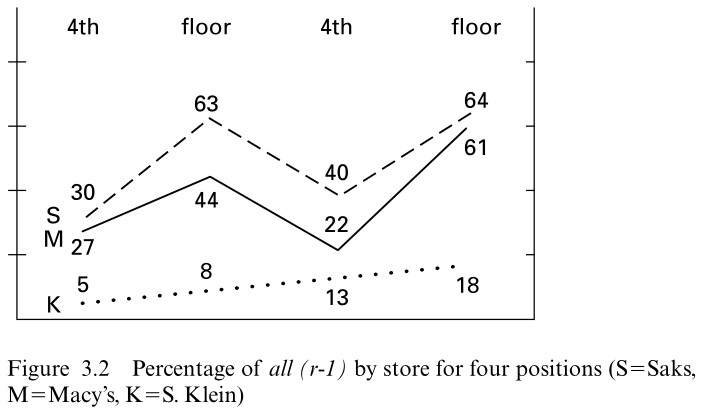
\includegraphics[scale=0.725]{department_store.jpg}
          \end{center}
        }
      \end{frame}

    \subsection{\subonethree}
      \begin{frame}{\subonethree}
        \begin{block}{}
          Variation according to age is treated as \alert{language change}:
          \begin{itemize}
            \item % Language change
The study of how languages change over time

          \end{itemize}
        \end{block}
        \begin{block}{Dubois and Horvath analyzed Cajun English linguistic variables by age} %\textcite{dubois_when_1999}
          \begin{itemize}
            \item (dh): whether speakers pronounced [ð] or [d]
            \item (th): whether speakers pronounced [θ] or [t]
          \end{itemize}
        \end{block}
        \begin{block}{}
          Would older or younger speakers be more likely to pronounce [d] and [t]?
        \end{block}
      \end{frame}

      \begin{frame}{\subonethree}
        \begin{center}
          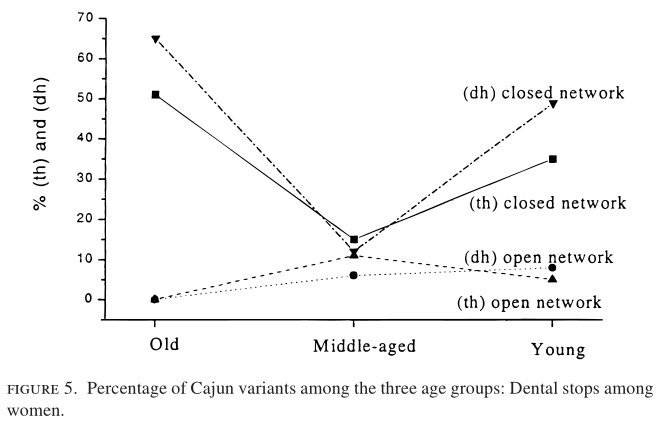
\includegraphics[scale=0.68]{cajun_fricatives_women.jpg}
        \end{center}
        \begin{block}{}
          What can we learn from this graph?
        \end{block}
      \end{frame}

      \begin{frame}{\subonethree}
        \begin{center}
          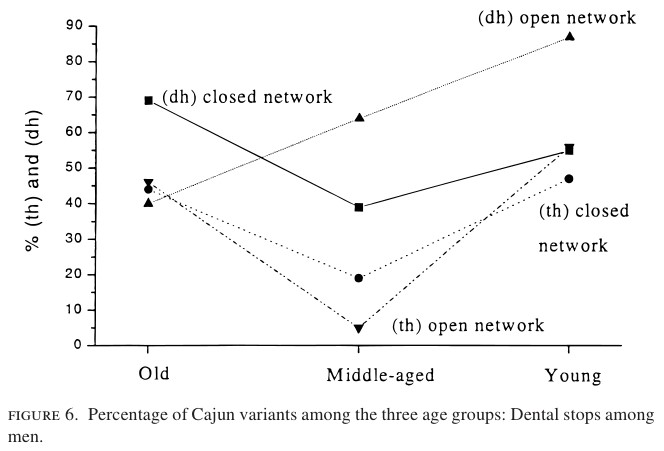
\includegraphics[scale=0.68]{cajun_fricatives_men.jpg}
        \end{center}
        \begin{block}{}
          Does this one for men tell us the same thing?
        \end{block}
      \end{frame}

    \subsection{\subonefour}
      \begin{frame}{\subonefour}
        \begin{definition}
          % Gender
One's identity in relation to varying conceptualizations of masculinity and femininity and the roles that may be attributed to those concepts

          \begin{itemize}
            \item A social construct, \emph{not} biological sex
          \end{itemize}
        \end{definition}
      \end{frame}

      \begin{frame}{\subonefour}
        \begin{columns}
          \column{0.5\linewidth}
            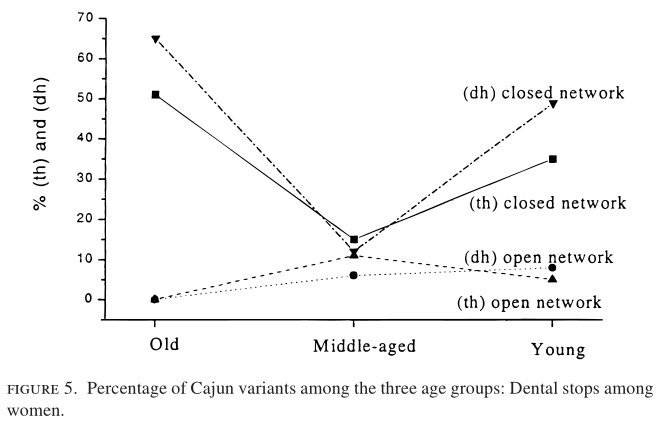
\includegraphics[scale=0.425]{cajun_fricatives_women.jpg}
          \column{0.5\linewidth}
            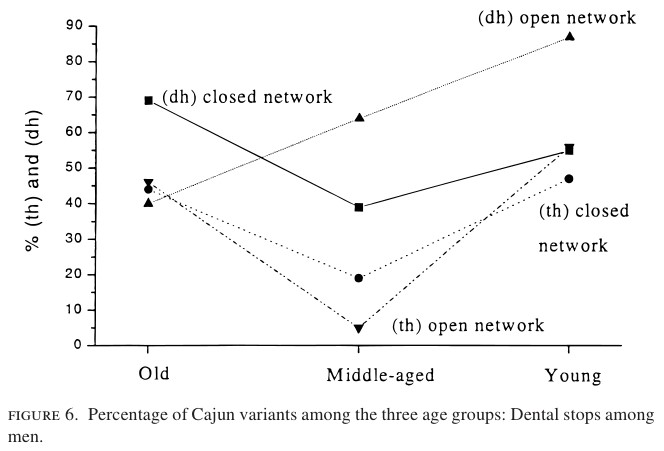
\includegraphics[scale=0.425]{cajun_fricatives_men.jpg}
        \end{columns}
        \begin{block}{}
          Overall, women used more standard variants
        \end{block}
      \end{frame}

      \begin{frame}{\subonefour}
        \begin{block}{This result is often found}
          \begin{itemize}
            \item Trudgill for (ing) in Norwich, England %\textcite{trudgill_social_1974}
            \item Eiskovits for negative concord in Australia %\textcite{collins_girl-talk_1989}
          \end{itemize}
        \end{block}
        \begin{block}{Why might women use standard variants more than men?}
          \uncover<2->{Some hypotheses:}
          \begin{itemize}
            \item<2-> Marginalized status $\rightarrow$ Overcompensate with language
            \item<2-> Role as primary caretakers $\rightarrow$ Use prestigious language for the children's sake
            \item<2-> Non-standard language is associated with masculinity
          \end{itemize}
        \end{block}
      \end{frame}

      \begin{frame}{References}
        % \printbibliography
      \end{frame}
\end{document}
